The source code in {\tt amrex/Src/Amr} contains a number of classes, most notably
{\tt Amr}, {\tt AmrLevel}, and {\tt LevelBld}.
These classes provide a more well developed set of tools for writing AMR codes
than the classes created for the {\tt Advection\_AmrCore} tutorial.
\begin{itemize}
\item The {\tt Amr} class is derived from {\tt AmrCore}, and manages data across the 
entire AMR hierarchy of grids.
\item The {\tt AmrLevel} class is a pure virtual class for managing data at a
single level of refinement.
\item The {\tt LevelBld} class is a pure virtual class for defining variable types
and attributes.
\end{itemize}

Many of our mature, publicly application codes contain derived classes that inherit directly
from {\tt AmrLevel}.  These include our compressible astrophysics code,
{\tt CASTRO},
(available in the {\tt AMReX-Astro/Castro} github repository) 
 and our computational cosmology code, {\tt Nyx}
(available in the {\tt AMReX-Astro/Nyx} github repository)   .
Our incompressible Navier-Stokes code, {\tt IAMR}
(available in the {\tt AMReX-codes/IAMR} github repository)
has a pure virtual class called {\tt NavierStokesBase} that inherits from {\tt AmrLevel},
and an additional derived class {\tt NavierStokes}.
Our low Mach number combustion code {\tt PeleLM} (not yet public) also inherits
from {\tt NavierStokesBase}.

The tutorial code in {\tt amrex/Tutorials/Amr/Advection\_AmrLevel} gives a simple
example of a class derived from {\tt AmrLevel} that can be used to solve
the advection equation on a subcycling-in-time AMR hierarchy.  Note that example
is essentially the same as the {\tt amrex/Tutorials/Amr/Advection\_AmrCore} tutorial
and documentation in Chapter \ref{Chap:AmrCore}, except now we use the provided
libraries in {\tt Src/Amr}.

The tutorial code also contains a {\tt LevelBldAdv} class (derived from {\tt LevelBld} in the
{\tt Source/Amr} directory).  This class is used to define variable types (how many, nodality,
interlevel interpolation stencils, etc.).

\section{{\tt Amr} Class}
The {\tt Amr} class is designed to manage parts of the computation  which do
not belong on a single level, like establishing and updating the hierarchy
of levels, global timestepping, and managing the different {\tt AmrLevel}s.
Most likely you will not need to derive any classes from {\tt Amr}.  Our mature
application codes use this base class without any derived classes.

One of the most important data members is an array of {\tt AmrLevel}s -
the {\tt Amr} class calls many functions from the {\tt AmrLevel} class to do
things like advance the solution on a level, compute a time step to be used 
for a level, etc.

\section{{\tt AmrLevel} Class}
Pure virtual functions include:
\begin{itemize}
\item {\tt computeInitialDt} Compute an array of time steps for each level of refinement.
Called at the beginning of the simulation.
\item {\tt computeNewDt} Compute an array of time steps for each level of refinement.
Called at the end of a coarse level advance.
\item {\tt advance} Advance the grids at a level.
\item {\tt post\_timestep} Work after at time step at a given level.  In this tutorial we do the 
AMR synchronization here.
\item {\tt post\_regrid} Work after regridding.  In this tutorial we redistribute particles.
\item {\tt post\_init} Work after initialization.  In this tutorial we perform AMR synchronization.
\item {\tt initData} Initialize the data on a given level at the beginning of the simulation.
\item {\tt init} There are two versions of this function used to initialize data on a level during regridding.  
One version is specifically for the case where the level did not previously exist (a newly created refined level)
\item {\tt errorEst} Perform the tagging at a level for refinement.
\end{itemize}

\subsection{{\tt StateData}}

The most important data managed by the {\tt AmrLevel} is an array of {\tt StateData},
which holds the scalar fields, etc., in the boxes that together make up the level.

{\tt StateData} is a class that essentially holds a pair of {\tt MultiFab}s: one at the old time and one
at the new time. {\tt AMReX} knows how to interpolate in time between these states to get data at
any intermediate point in time. The main data that we care about in our applications codes 
(such as the fluid state) will be stored as {\tt StateData}. Essentially, data is made {\tt StateData}
if we need it to be stored in checkpoints / plotfiles, and/or we want it to be automatically
interpolated when we refine.
An {\tt AmrLevel} stores an array of {\tt StateData} (in a C ++ array called state). We index this array
using integer keys (defined via an enum in, e.g., {\tt AmrLevelAdv.H}):
\begin{lstlisting}[language=cpp]
enum StateType { Phi_Type = 0,
                 NUM_STATE_TYPE };
\end{lstlisting}
In our tutorial code, we use the function {\tt AmrLevelAdv::variableSetup} to tell our simulation about
the {\tt StateData} (e.g., how many variables, ghost cells, nodality, etc.)
Note that if you have more than one {\tt StateType}, each of the different {\tt StateData} 
carried in the state array can have different numbers
of components, ghost cells, boundary conditions, etc. This is the main reason we separate all this
data into separate {\tt StateData} objects collected together in an indexable array.

\section{{\tt LevelBld} Class}
The {\tt LevelBld} class is a pure virtual class for defining variable types
and attributes.  To more easily understand its usage, refer to the derived class,
{\tt LevelBldAdv} in the tutorial.  The {\tt variableSetUp} and {\tt variableCleanUp} are implemented,
and in this tutorial call routines in the {\tt AmrLevelAdv} class, e.g.,
\begin{lstlisting}[language=cpp]
void
AmrLevelAdv::variableSetUp ()
{
    BL_ASSERT(desc_lst.size() == 0);

    // Get options, set phys_bc
    read_params();

    desc_lst.addDescriptor(Phi_Type,IndexType::TheCellType(),
                           StateDescriptor::Point,0,NUM_STATE,
			   &cell_cons_interp);

    int lo_bc[BL_SPACEDIM];
    int hi_bc[BL_SPACEDIM];
    for (int i = 0; i < BL_SPACEDIM; ++i) {
	lo_bc[i] = hi_bc[i] = INT_DIR;   // periodic boundaries
    }
    
    BCRec bc(lo_bc, hi_bc);

    desc_lst.setComponent(Phi_Type, 0, "phi", bc, 
			  StateDescriptor::BndryFunc(nullfill));
}
\end{lstlisting}
We see how to define the {\tt StateType}, including nodality, whether or not we want
the variable to represent a point in time or an interval over time (useful for returning
the time associated with data), the number of ghost cells, number of components,
and the interlevel interpolation (See {\tt AMReX\_Interpolator} for various interpolation
types.  We also see how to specify physical boundary functions by providing a function (in this case,
{\tt nullfill} since we are not using physical boundary conditions), where {\tt nullfill} is
defined in a fortran routine in the tutorial source code.

\section{{\tt Advection\_AmrLevel} Example}

Figure \ref{fig:AmrAdvection_AmrLevel_flowchart} shows a source
code tree for the {\tt AmrAdvection\_AmrLevel} example.
%%%%%%%%%%%%%%%%%%%%%%%%%%%%%
\begin{figure}[htb]
\begin{center}
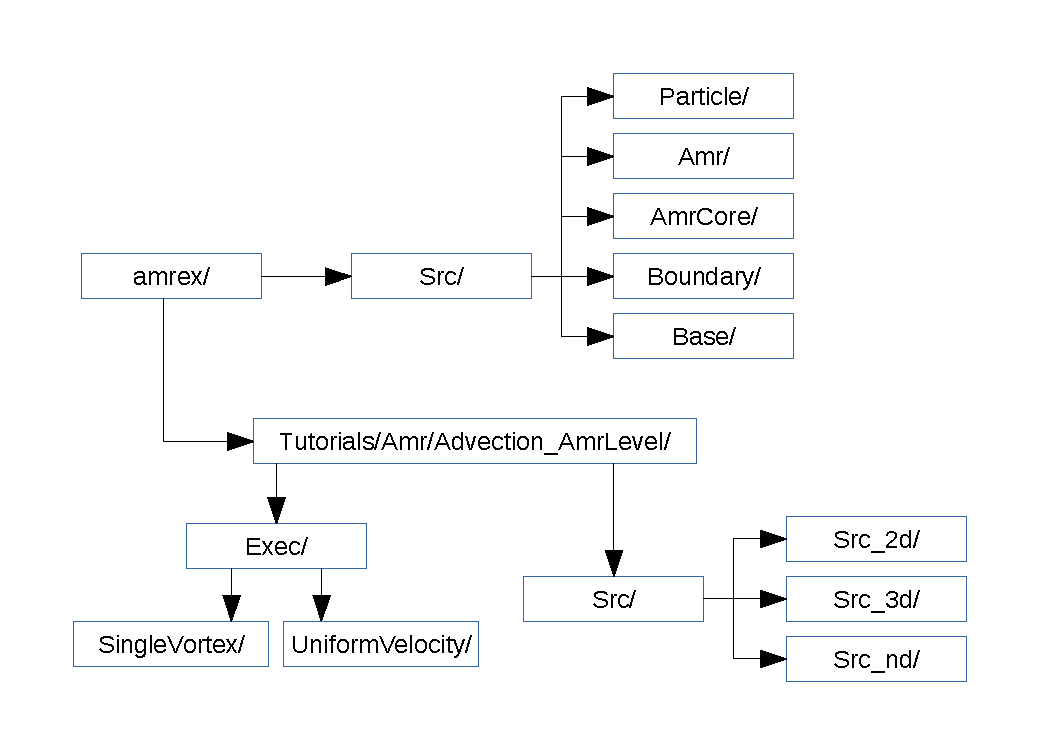
\includegraphics[width=4in]{./AmrLevel/figs/flowchart.pdf}
\caption{\label{fig:AmrAdvection_AmrLevel_flowchart} Source code tree for the 
         {\tt AmrAdvection\_AmrLevel} example.}
\end{center}
\end{figure}
%%%%%%%%%%%%%%%%%%%%%%%%%%%%%
\begin{itemize}
\item {\tt amrex/Src/}
\begin{itemize}
\item {\tt Base/} Base {\tt amrex} library.
\item {\tt Boundary/} An assortment of classes for handling boundary data.
\item {\tt AmrCore/} AMR data management classes, described in more detail above.
\item {\tt Amr/}
\end{itemize}
\item {\tt Advection\_AmrLevel/Src} Source code specific to this example.  Most notably
is the {\tt AmrLevelAdv} class, which is derived from {\tt AmrLevel}.  The subdirectories {\tt Src\_2d}
and {\tt Src\_3d} contain dimension specific routines.  {\tt Src\_nd} contains dimension-independent routines.
\item {\tt Exec} Contains a makefile so a user can write other examples besides {\tt SingleVortex} and {\tt UniformVelocity}.
\item {\tt SingleVortex} and {\tt UniformVelocity}
Build the code here by editing the {\tt GNUmakefile} and running {\tt make}.  There
is also problem-specific source code here used for initialization or specifying the velocity field used in this
simulation.
\end{itemize}

\begin{lstlisting}[language=cpp]
/* Advection_AmrLevel Pseudocode */
main()
  Amr amr;
  amr.init()
  loop { 
    amr.coarseTimeStep()
      /* compute dt */
      timeStep()
        amr_level[level]->advance()
        /* call timeStep r times for next-finer level */
        amr_level[level]->post_timestep() // AMR synchronization
      postCoarseTimeStep()
      /* write plotfile and checkpoint */
  }
  /* write final plotfile and checkpoint */
\end{lstlisting}


\section{Particles}
There is an option to turn on passively advected particles.  In the {\tt GNUmakefile},
add the line ``{\tt USE\_PARTICLES = TRUE}'' and build the code 
(do a {\tt make realclean} first).
In the inputs file, add the line ``{\tt adv.do\_tracers = 1}''.
When you run the code, within each plotfile directory there will be a subdirectory
called ``Tracer''.

Copy the files from {\tt amrex/Tools/Py\_util/amrex\_particles\_to\_vtp} into
the run directory and type, e.g.,\\ \\
{\tt python amrex\_binary\_particles\_to\_vtp.py plt00000 Tracer}\\ \\
To generate a vtp file you can open with \paraview\
(Refer to Chapter \ref{Chap:Visualization}).

